\documentclass{article}

\usepackage[left=2cm,right=2cm,top=2cm,bottom=2cm]{geometry} 

\usepackage[utf8]{inputenc}   % otra alternativa para los caracteres acentuados y la "ñ"
\usepackage[           spanish % para poder usar el español
                      ,es-tabla % para los captions de las tablas
                       ]{babel}   
\decimalpoint %para usar el punto decimal en vez de coma para los números con decimales

%\usepackage{beton}
%\usepackage[T1]{fontenc}

\usepackage{parskip}
\usepackage{xcolor}

\usepackage{caption}

\usepackage{fancyvrb}

\usepackage{enumerate} % paquete para poder personalizar fácilmente la apariencia de las listas enumerativas

\usepackage{graphicx} % figuras
\usepackage{subfigure} % subfiguras

\usepackage{amsfonts}
\usepackage{amsmath}

\usepackage[formats]{listings}
\lstdefineformat{R}{~=\( \sim \)}
\lstset{basicstyle=\ttfamily,format=R}

\definecolor{gris}{RGB}{220,220,220}
	
\usepackage{float} % para controlar la situación de los entornos flotantes

\restylefloat{figure}
\restylefloat{table} 
\setlength{\parindent}{0mm}


\usepackage[bookmarks=true,
            bookmarksnumbered=false, % true means bookmarks in 
                                     % left window are numbered
            bookmarksopen=false,     % true means only level 1
                                     % are displayed.
            colorlinks=true,
            allcolors=blue,
            urlcolor=blue]{hyperref}
\definecolor{webblue}{rgb}{0, 0, 0.5}  % less intense blue


\title{\Huge SWAP: Balanceo de carga en un sitio web\vspace{10mm}}

\author{\huge David Cabezas Berrido \vspace{10mm} \\ 
  \huge dxabezas@correo.ugr.es \vspace{10mm}}

\begin{document}
\maketitle
\tableofcontents
\newpage

\section{Preparativos}

Creamos dos archivos \texttt{/var/www/html/index.html} básicos en las máquinas 1 y 2, donde se referencie el número de la máquina a la que
pertenece el archivo para saber cuál de las dos máquinas atendió la petición.

Creamos una nueva máquina virtual M3 con Ubuntu Server, pero no instalamos los servicios de la práctica 1, ya que no podemos
tener a Apache ocupando el puerto 80. Nos limitamos a configurar el doble
adaptador de red como hicimos en las otras dos máquinas. Su dirección IP es 192.168.56.103, para hacer peticiones desde la
máquina anfitriona.

A partir de aquí, todas las órdenes y configuraciones se realizan en M3 a menos que digamos
lo contrario.

\section{Balanceo de carga con NGINX}

Comenzamos instalando y lanzando NGINX:

\begin{verbatim}
	sudo apt-get update && sudo apt-get dist-upgrade && sudo apt-get autoremove
	sudo apt-get install nginx
	sudo systemctl start nginx
\end{verbatim}

Comprobamos que el servicio está en funcionamiento.

\begin{figure}[H]
	\centering
	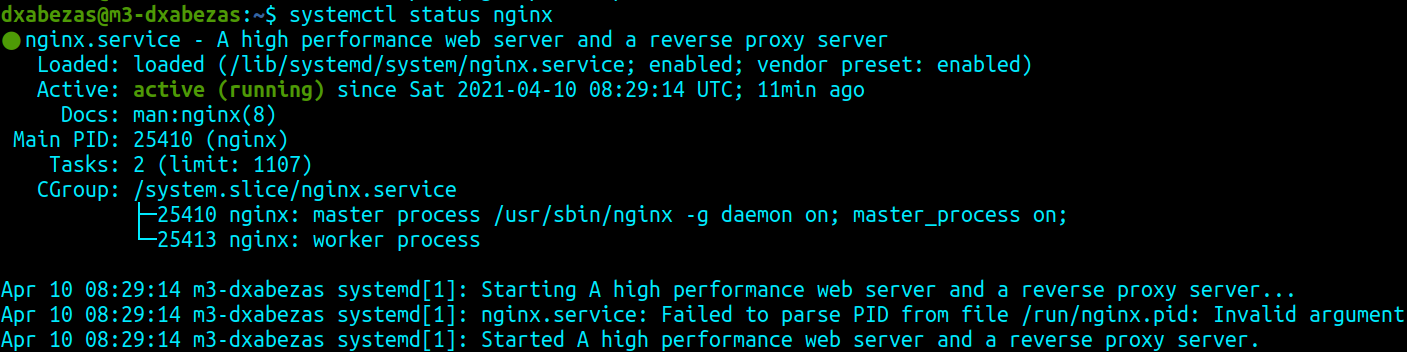
\includegraphics[width=148mm]{imgs/nginx-status}
	\caption{NGINX está activo.}
	\label{fig:nginx-status}
\end{figure}

Escribimos en \texttt{/etc/nginx/conf.d/default.conf} la configuración que se indica en el guión
para que NGINX funcione como balanceador de carga en lugar de como servidor web.

\begin{Verbatim}[tabsize=4]
upstream balanceo_dxabezas {
	server 192.168.56.101;
	server 192.168.56.102;
}

server{
	listen 80;
	server_name balanceador_dxabezas;
	access_log /var/log/nginx/balanceador_dxabezas.access.log;
	error_log /var/log/nginx/balanceador_dxabezas.error.log;
	root /var/www/;

	location /
	{
		proxy_pass http://balanceo_dxabezas;
		proxy_set_header Host $host;
		proxy_set_header X-Real-IP $remote_addr;
		proxy_set_header X-Forwarded-For $proxy_add_x_forwarded_for;
		proxy_http_version 1.1;
		proxy_set_header Connection "";
	}
}
\end{Verbatim}

Reestauramos el servicio con \verb^sudo service nginx restart^, haremos esto (aunque no lo digamos) cada vez que
modifiquemos este fichero. Ahora si visitamos la IP de M3
en el navegador de la máquina anfitriona, observamos que NGINX sigue funcionando como servidor
web.

\begin{figure}[H]
	\centering
	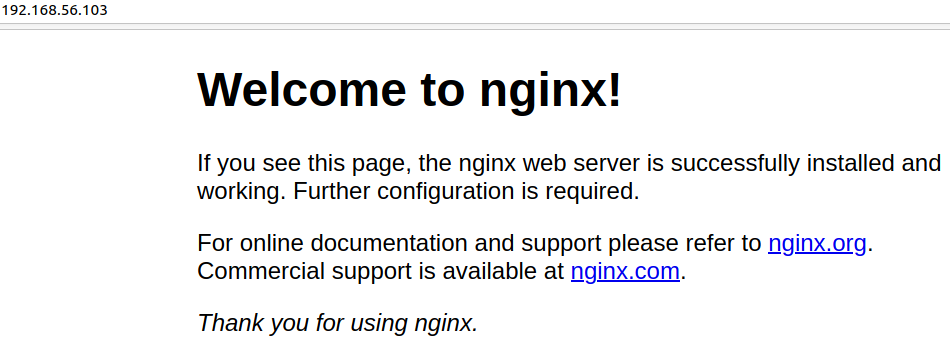
\includegraphics[width=100mm]{imgs/nginx-web}
	\caption{NGINX está funcionando como servidor web.}
	\label{fig:nginx-web}
\end{figure}

Como se nos indica en el guión, comentamos la línea \verb^/etc/nginx/sites-enabled/*;^
del fichero \texttt{/etc/nginx/nginx.conf}. Ahora accedemos a la IP de la máquina 3, y cada vez que refrestamos la página
se turnan las máquinas 1 y 2 para servirnos su \texttt{index.html}.

\begin{figure}[H]
	\centering
	\subfigure{
\includegraphics[width=120mm]{imgs/index-m1}}
	\subfigure{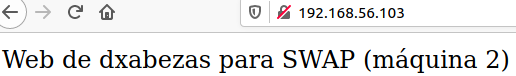
\includegraphics[width=120mm]{imgs/index-m2}}
	\label{fig:index}
\end{figure}

Ahora añadimos el parámetro \texttt{weight} en el fichero \texttt{/etc/nginx/conf.d/default.conf} para que la máquina 2 reciba
el doble de peticiones que la 1.

\begin{Verbatim}[tabsize=4]
upstream balanceo_dxabezas {
	server 192.168.56.101 weight=1;
	server 192.168.56.102 weight=2;
}
\end{Verbatim}
Si ahora vamos refrescando la página, la máquina que nos atiende en cada momento es: \\
M1, M2, M2, M1, M2, M2, M1, M2, M2, \ldots

Seguidamente, probamos a cambiar el algoritmo de Round-Robin (por defecto) a IP-HASH para que siempre nos atienda la misma máquina,
lo conseguimos añadiendo la directiva \texttt{ip\_hash} en el fichero de configuración.
\begin{Verbatim}[tabsize=4]
upstream balanceo_dxabezas {
	ip_hash;
	server 192.168.56.101;
	server 192.168.56.102;
}
\end{Verbatim}
Ahora, por más que refresquemos la página, nos atiende siempre la misma máquina, en nuestro caso la 2. 

Finalmente, activamos las conexiones con keepalive the 3 segundos.
\begin{Verbatim}[tabsize=4]
upstream balanceo_dxabezas {
	server 192.168.56.101;
	server 192.168.56.102;
	keepalive 3;
}
\end{Verbatim}
Aunque no es sencillo comprobar que funciona correctamente, ya que recargar la página abre una conexión nueva.

Probamos algunas opciones avanzadas más. De las propuestas en el guión, elegiremos aquellas cuyo
funcionamiento podamos comprobar más fácilmente.

\begin{Verbatim}[tabsize=4]
upstream balanceo_dxabezas {
	ip_hash;
	server 192.168.56.101;
	server 192.168.56.102 down;
}
\end{Verbatim}
Marcando M2 como \texttt{down} con \texttt{ip\_hash}, comprobamos que ahora nos atiende M1 en lugar de M2.

\begin{Verbatim}[tabsize=4]
upstream balanceo_dxabezas {
	server 192.168.56.101;
	server 192.168.56.102 backup;
}
\end{Verbatim}
Ahora marcamos M2 como backup y siempre nos atiende M1. Si desactivamos el servicio de M1 con \\
\verb^sudo systemctl stop apache2^, pasa a atendernos todo el rato M2.

\section{Balanceo de carga con HAProxy}

Primero apagamos NGINX para que libere el puerto 80 con \verb^sudo systemctl stop nginx^

Instalamos el balanceador con \verb^sudo apt install haproxy^. Añadimos la siguiente configuración al fichero \\
\texttt{/etc/haproxy/haproxy.cfg}, y hacemos \verb^sudo systemctl restart haproxy.service^ (lo haremos tras cada
modificación del fichero de configuración).

\begin{Verbatim}[tabsize=4]
frontend http-in
	bind *:80
	default_backend balanceo_dxabezas

backend balanceo_dxabezas
	server  m1 192.168.56.101:80 maxconn 32
	server  m2 192.168.56.102:80 maxconn 32
\end{Verbatim}

Si ahora hacemos \texttt{status}, vemos que el servicio está activo y nuestro balanceador iniciado.

\begin{figure}[H]
	\centering
	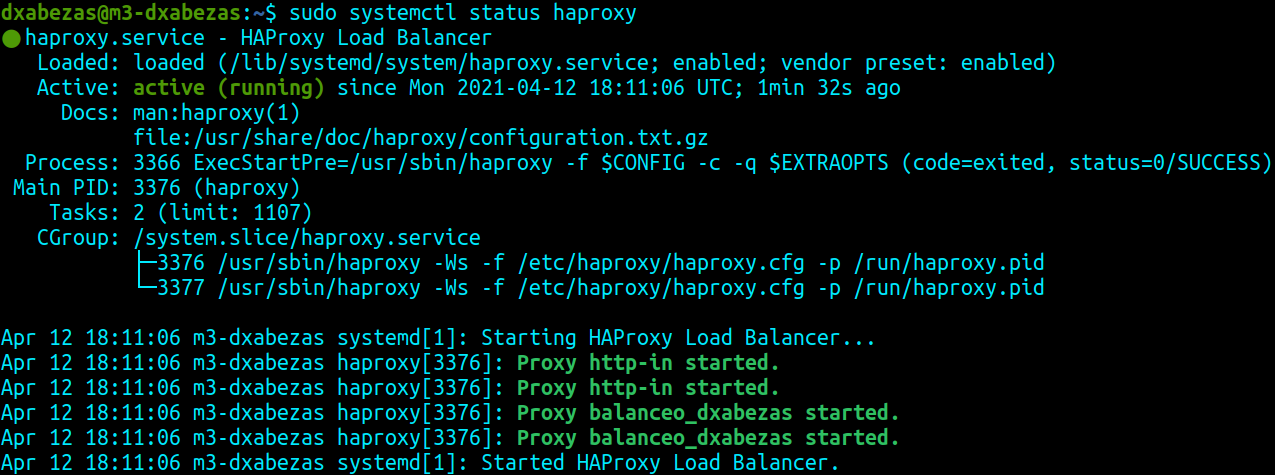
\includegraphics[width=160mm]{imgs/haproxy-status}
	\label{fig:haproxy-status}
\end{figure}

Si ahora accedemos a \texttt{192.168.56.103} desde el navegador, observamos que las dos máquinas se turnan para
servirnos su \texttt{index.html}.

Ahora configuramos la ponderación.

\begin{Verbatim}[tabsize=4]
frontend http-in
	bind *:80
	default_backend balanceo_dxabezas

backend balanceo_dxabezas
	server  m1 192.168.56.101:80 maxconn 32 weight 2
	server  m2 192.168.56.102:80 maxconn 32 weight 1
\end{Verbatim}
Si refrescamos la página nos atiende M1, M1, M2, M1, M1, M2, M1, M1, M2, \ldots

Ahora buscaremos algunas opciones avanzadas. Seleccionamos balanceo por IP-HASH. 

\begin{Verbatim}[tabsize=4]
frontend http-in
	bind *:80
	default_backend balanceo_dxabezas

backend balanceo_dxabezas
	balance source
	hash-type consistent
	server  m1 192.168.56.101:80 maxconn 32
	server  m2 192.168.56.102:80 maxconn 32
\end{Verbatim}
Ahora nos atiende siempre M1.
    
Finalmente, ponemos M1 en modo \texttt{backup}. Debemos añadir \texttt{check}, ya que no se activa el servidor de
backup si \texttt{check} no devuelve \texttt{DOWN}. Si no añadimos la comprobación, las peticiones no son atendidas.
\begin{Verbatim}[tabsize=4]
frontend http-in
	bind *:80
	default_backend balanceo_dxabezas

backend balanceo_dxabezas
	server  m1 192.168.56.101:80 maxconn 32 check backup
	server  m2 192.168.56.102:80 maxconn 32 check
\end{Verbatim}
Nos atiende siempre M2, pero cuando apagamos el servicio Apache2 en M2, pasa a atendernos siempre M1.

\section{Estadísticas de HAProxy}

Dejamos la configuración con Round-Robin básico, pero mantenemos los \texttt{check}.

Ahora añadimos la siguiente configuración (a HAProxy) para habilitar las estadísticas: En \texttt{global} escribimos
\verb^stats socket /var/lib/haproxy/stats^, sustituyéndo la anterior línea de \texttt{stats socket}; y añadimos el
siguiente bloque:
\begin{Verbatim}[tabsize=4]
listen stats
	bind *:9999
	mode http
	stats enable
	stats uri /stats
	stats realm HAProxy\ Statistics
	stats auth dxabezas:dxabezas
\end{Verbatim}
Reseteamos el servicio. Ahora, en la ruta \texttt{/stats} del puerto 9999 podemos ver las estadísticas,
logueandonos primero con \texttt{dxabezas} tanto como usuario como contraseña.

\begin{figure}[H]
	\centering
	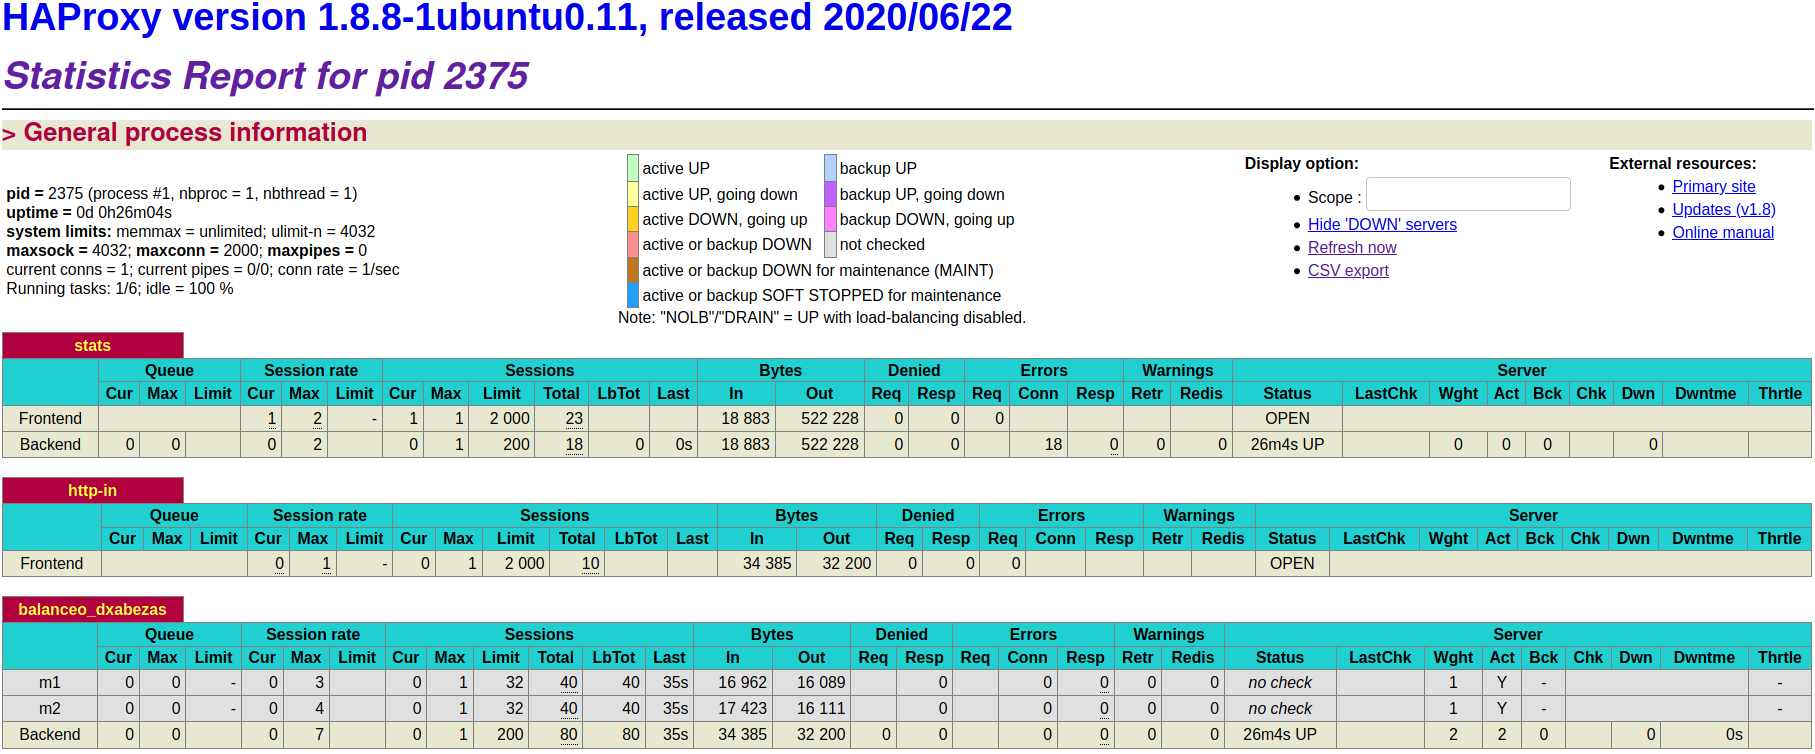
\includegraphics[width=170mm]{imgs/stats-dashboard}
	\caption{Estadísticas de HAProxy, podemos ver los pesos de cada servidor, las sesiones totales,
		las sesiones actualtes de cada servidor (Cur=0), el máximo (1) y el límite de sesiones
		 concurrentes (\texttt{maxconn 32}); también el tiempo que llevan funcionando.}
	\label{fig:stats-dashboard}
\end{figure}

Añadiendo estas dos líneas a \verb^listen stats^ y restaurando el servicio, hacemos que los datos se refresquen
cada 15 segundos, y que podamos modificar marcar los servidores como DOWN o MAINTENANCE, o cortar sus sesiones
actuales.
\begin{Verbatim}[tabsize=4]
	stats refresh 15s
	stats admin if TRUE
\end{Verbatim}

\begin{figure}[H]
	\centering
	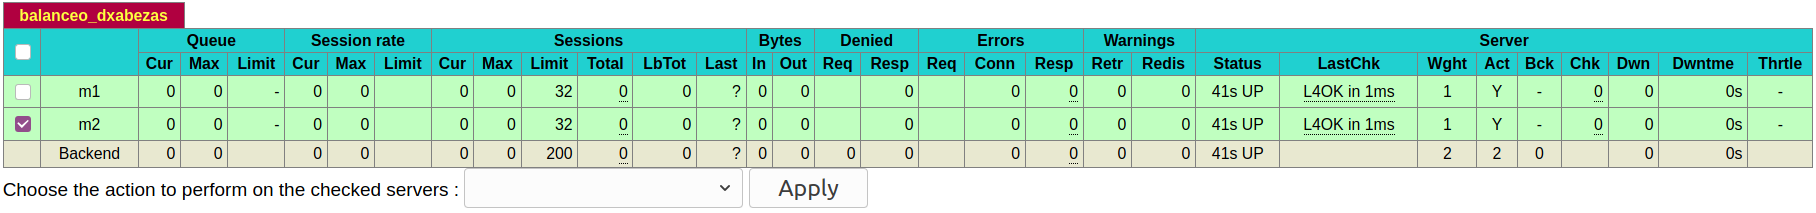
\includegraphics[width=170mm]{imgs/stats-admin}
	\caption{Podemos elegir acciones que aplicar a los servidores que marcamos.}
	\label{fig:stats-admin}
\end{figure}

\section{Balanceo de carga con Pound}

Descargamos el programa de aquí:
\href{https://packages.ubuntu.com/xenial-updates/amd64/pound/download}{https://packages.ubuntu.com/xenial-updates/amd64/pound/download}.

Ahora nos vamos al fichero de configuración \texttt{/etc/pound/pound.cfg} y escribimos lo siguiente:
\begin{Verbatim}[tabsize=4]
ListenHTTP
	Address 192.168.56.103
	Port    80
End

Service
	BackEnd
		Address 192.168.56.101
		Port    80
		Priority        2
	End

	BackEnd
		Address 192.168.56.102
		Port    80
		Priority        1
	End
End
\end{Verbatim}
Además, hay que cambiar \texttt{startup=0} por \texttt{startup=1}, en el fichero \texttt{/etc/default/pound}
como se indica en el siguiente mensaje de estado (sale cortado): 
\begin{figure}[H]
	\centering
	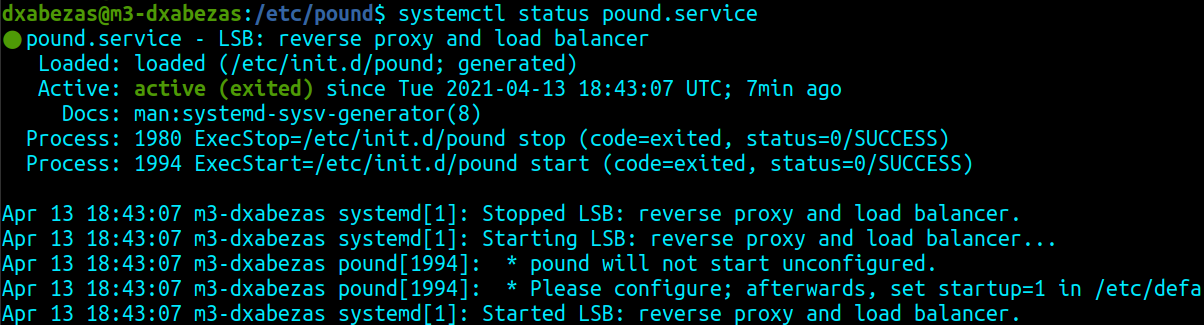
\includegraphics[width=150mm]{imgs/pound-status}
	\caption{El servicio no arrancará hasta que no se marque como configurado.}
	\label{fig:pound-status}
\end{figure}
Hemos aprovechado para poner ponderaciones con \texttt{Priority}. Nos conectamos a la IP de M3 desde el
navegador y nos M1 atiende el doble de peticiones que M2.

Se pueden poner más opciones como \texttt{TimeOut 10}, para fijar un tiempo de TimeOut de 10 segundos
antes de que Pound considere que el servidor no va a responder.

Como opción avanzada, introducimos \texttt{Emergency}, para que sólo use el servidor cuando el resto falle.
\begin{Verbatim}[tabsize=4]
Service
	BackEnd
		Address 192.168.56.101
		Port    80
	End

	Emergency
		Address 192.168.56.102
		Port    80
	End
End
\end{Verbatim}
Ahora nos atiende siempre M1, pero si apagamos el servicio Apache2 en M1 pasa a atendernos M2.

Finalmente, Pound tiene una funcionalidad similar al IP-Hash llamada \texttt{Session}, que hace que las
peticiones provenientes de la misma IP sean atendidas por la misma máquina dentro de un tiempo, a partir
del cual se descarta la sesión. Dejamos la configuración de esta forma:
\begin{Verbatim}[tabsize=4]
Service
	BackEnd
		Address 192.168.56.101
		Port    80
	End

	BackEnd
		Address 192.168.56.102
		Port    80
	End
	
	Session
		Type IP
		TTL 60
	End
End
\end{Verbatim}
Las peticiones de la misma IP siempre son atendidas por al misma máquina. Tras 60 segundos sin peticiones, se
descarta la sesión.

\section{Someter a carga la granja web con AB}

Apache Benchmark se instala con el servicio Apache2, lo instalo en mi máquina anfitriona, desde la que lanzaré
peticiones a M3.

Lanzamos el benchmark desde la máquina anfitriona. Lanzamos 10000 peticiones con un nivel de concurrencia de 10.

\begin{Verbatim}[tabsize=4]
ab -n 10000 -c 10 http://192.168.56.103/index.html
\end{Verbatim}

Observamos con \texttt{top} como Apache2 se convierte en el proceso que más recursos consume de M1 Y M2, y 
el balanceador el que más consume de M3.

\begin{figure}[H]
	\centering
	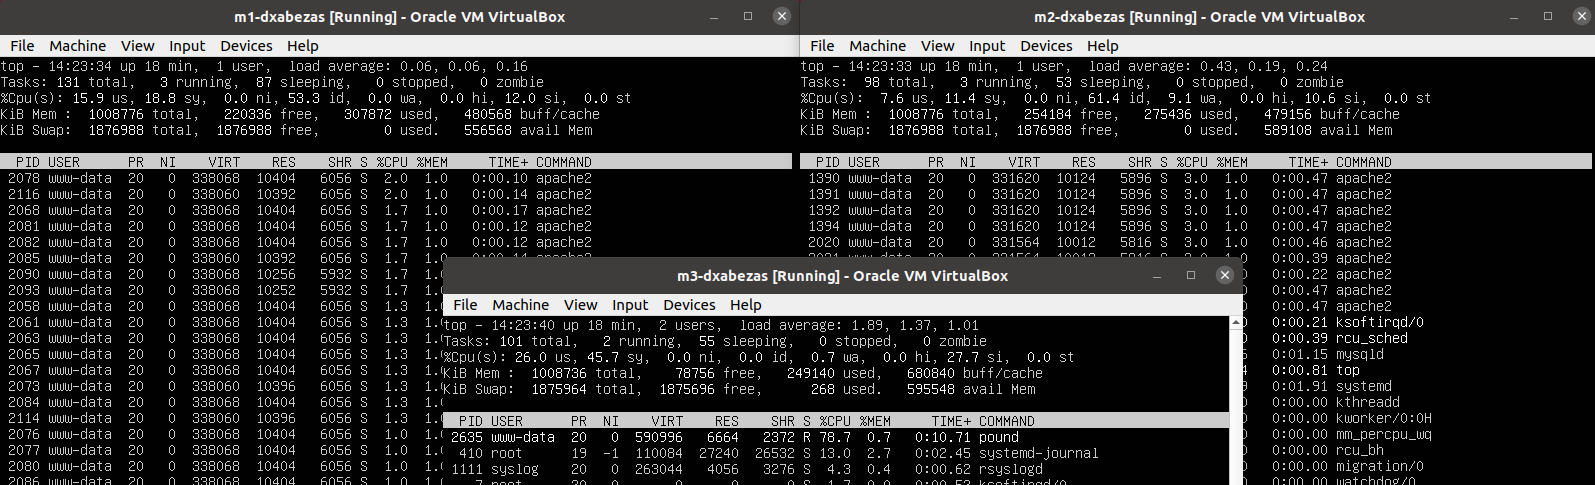
\includegraphics[width=170mm]{imgs/top}
	\caption{Ante la llegada masiva de peticiones, los servicios empiezan a consumir más recursos.}
	\label{fig:top}
\end{figure}

Esperamos unos segundos, y AB nos genera un informe sobre el rendimiento del servidor.

\begin{figure}[H]
	\centering
	\subfigure{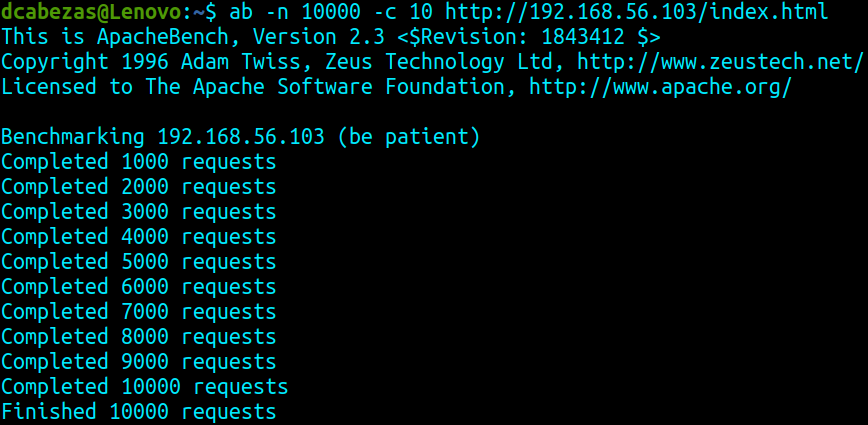
\includegraphics[width=130mm]{imgs/ab-1}}
\end{figure}\begin{figure}[H]\ContinuedFloat
	\subfigure{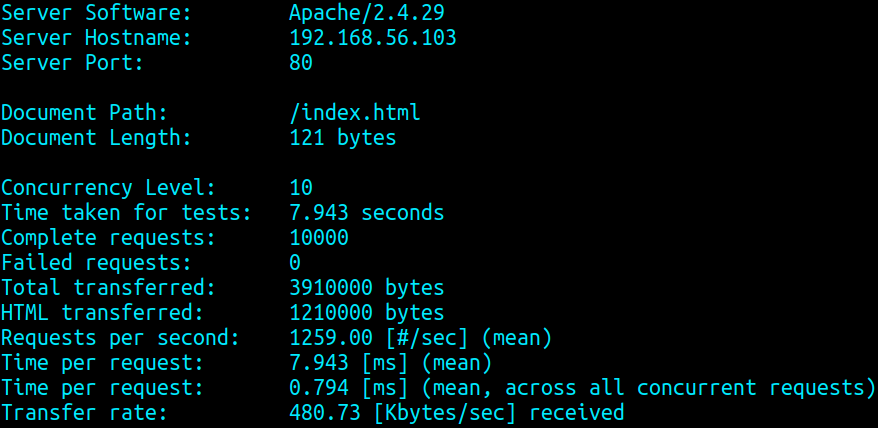
\includegraphics[width=90mm]{imgs/ab-2}}
	\subfigure{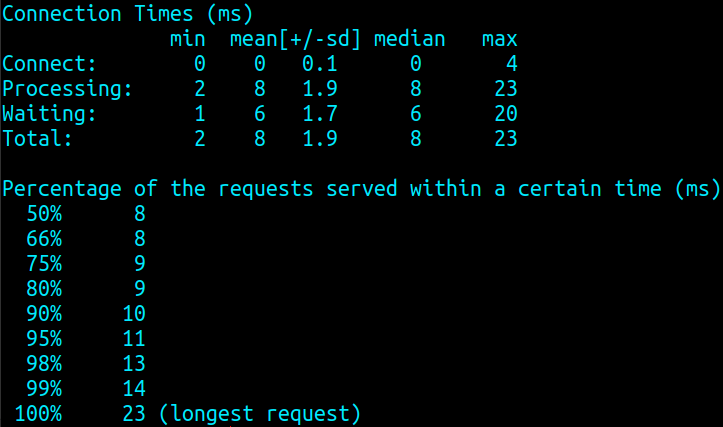
\includegraphics[width=80mm]{imgs/ab-3}}
	\caption{Salida de Apache Benchmark. In la primera imagen nos informa del progreso de benchmarking. En
	la segunda imagen tenemos información sobre el servidor y el fichero solicitado (\texttt{index.html}), así como
del número de peticiones y bytes transferidos y el tiempo tomado. En la tercera imagen tenemos estadísticas sobre
los tiempos que toma la conexión, procesamiento y espera de las peticiones, y también los milisegundos bajo los cuales
se han atendido distintos porcentajes de peticiones.}
	\label{fig:ab}
\end{figure}
Aunque vayamos a utilizar el criterio peticiones/segundo (en este caso 1259, segunda imagen) para comparar los balanceadores, 
también son muy interesantes
las medias de la tercera imagen. Nos permiten ``asegurar'' que nuestro servidor atiende cierto porcentaje de las peticiones
en cierto tiempo. Ej: ``Generalmente, ninguna petición tarda en antenderse más de 23 ms'',
``El 99\% de las peticiones que recibe son atendidas en 14 segundos o menos''.

Por último, introduciremos algunas opciones y parámetros de Apache Benchmark que pueden ser útiles.
\begin{itemize}
	\item \texttt{-e archivo.csv} genera un archivo CSV con los datos de la segunda mitad de la tercera imagen.
	\item \texttt{-q} elimina los mensajes de progreso.
	\item \texttt{-t 60} indica el número máximo de segundos que durará el benchmark aunque no se completen todas
	las peticiones, en este caso 60.
	\item \texttt{-p archivo} para hacer peticiones de POST de un archivo.
	\item \texttt{-u archivo} para hacer peticiones de PUT de un archivo.
	\item \texttt{-T content-type} indica el header para POST y PUT, es obligatorio si se usa alguna de las dos opciones anteriores.
\end{itemize}

\section{Balanceo de carga con Gobetween}

Instalamos Gobetween desde la Snap Store de Ubuntu, que viene instalada y habilitada por defecto.
\begin{Verbatim}[tabsize=4]
sudo snap install gobetween --edge
\end{Verbatim}

Como lo hemos instalado desde Snap, tenemos que invocarlo con
\begin{Verbatim}[tabsize=4]
/snap/gobetween/current/bin/gobetween
\end{Verbatim}

Creamos un fichero de configuración en \texttt{/snap/gobetween/gobetween-cfg.toml}.
\begin{Verbatim}[tabsize=4]
[servers.sample]
bind = "192.168.56.103:80"
protocol = "tcp"
balance = "roundrobin"

max_connections = 10000
client_idle_timeout = "10m"
backend_idle_timeout = "10m"
backend_connection_timeout = "2s"

[servers.sample.discovery]
kind = "static"
static_list = [
	"192.168.56.101:80",
	"192.168.56.102:80"
]

[servers.sample.healthcheck]
fails = 1
passes = 1
interval = "2s"
kind = "ping"
ping_timeout_duration = "500ms"
\end{Verbatim}
Ahora lo lanzamos con el siguiente comando, y efectivamente funciona. Hemos necesitado lanzarlo con sudo porque
se le denegaba el acceso de escucha en el puerto 80.

\begin{figure}[H]
	\centering
	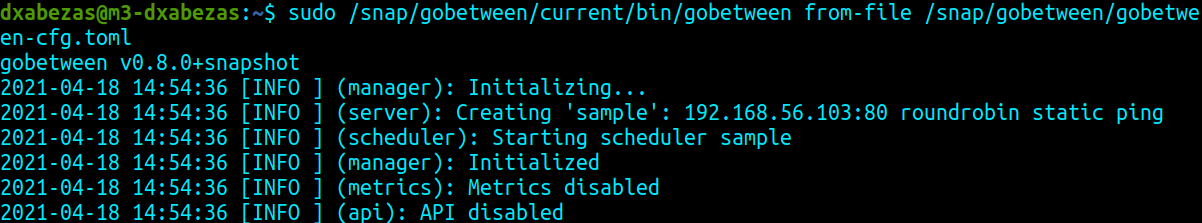
\includegraphics[width=160mm]{imgs/gobetween}
	\caption{Lanzamos Gobetween indicando el fichero de configuración.}
	\label{fig:gobetween}
\end{figure}

El parámetro balance indica el algoritmo para distribuir la carga, también puede ser \texttt{iphash} (IP-Hash),
\texttt{leastconn} (menor número de conexiones) o \texttt{weight} (ponderaciones). Este último nos obliga a escribir la
lista de servidores con el siguiente formato.
\begin{Verbatim}[tabsize=4]
[servers.sample.discovery]
kind = "static"
static_list = [
	"192.168.56.101:80 weight=2",
	"192.168.56.102:80 weight=1"
]
\end{Verbatim}

En el último bloque del fichero de configuración sirve para hacer comprobaciones del estado de los servidores.
En este caso, el balanceador hará \texttt{ping} cada dos segundos, y se espera una respuesta del servidor en 500
milisegundos. Tras un fallo (parámetro \texttt{fails}), se marca el servidor como DOWN, pero se siguen enviando pings
por si en algún momento se recibe respuesta. Con una respuesta (parámetro \texttt{passes}) se vuelve a marcar el
servidor como OK.

\section{Balanceo de carga con Zevenet}

TODO: adaptadores, seleccionar host-only el bueno durante instalación
TODO: configuraciones en puerto 4444

m4zevenet.org

\section{Análisis comparativo de distintos balanceadores}

En la siguiente tabla recogemos las peticiones por segundo de cada balanceador con cada algoritmo para un benchmark
como el anterior, con 10000 peticiones y concurrencia 10.

Cabe destacar que no estamos seguros de que Pound haga Round Robin por defecto. De hecho sospecho que no, puesto que
a veces nos atiende dos veces seguidas la misma máquina. Por tanto, el nombre de la columna Round Robin debería ser
Predeterminado.

También para Pound utilizamos Session en lugar de IP-Hash,
ambos comparten el objetivo de que varias peticiones de la misma IP sean atendidas por la misma máquina.

\begin{table}[H]
	\centering
	\begin{tabular}{|c|c|c|}
		\hline
		\multicolumn{1}{|l|}{peticiones/s} & \multicolumn{1}{l|}{Round-Robin} & \multicolumn{1}{l|}{IP-Hash / Session} \\ \hline
		NGINX                              & 1946.2                           & 2119.05                                \\ \hline
		HAProxy                            & 1666.1                           & 1718.69                                \\ \hline
		Pound                              & 1259                             & 1185.1                                 \\ \hline
		Gobetween                            & 1421.19                  & 1364.69                                \\ \hline
	\end{tabular}
\end{table}

TODO: session mucho más lento que IP-Hash
TODO: grafico de barras

\end{document}
